%\documentclass[AER  , draftmode]{AEA}
\documentclass[11pt, a4paper]{article}
\usepackage[nohead]{geometry}
\geometry{left=1in,right=1in,top=1in,bottom=1in} % set margins


\usepackage{soul}
\usepackage{natbib}
\usepackage{graphicx}             
\graphicspath{{./paper/Figuras/}}
\usepackage{hyperref}

\usepackage{float}                
\usepackage{amsmath}
\usepackage{amscd}
\usepackage{amsfonts}
\usepackage{amssymb}
\usepackage{bbm}
\usepackage{booktabs}
\usepackage{nameref}
\usepackage{multirow}
\usepackage[nokeyprefix]{refstyle}
\usepackage{rotating}
\usepackage{threeparttable}
\usepackage{lscape}
\usepackage{enumerate}
\usepackage{afterpage}
\usepackage{caption}
\usepackage{subcaption}
\usepackage{epstopdf}
\usepackage{comment}


\epstopdfDeclareGraphicsRule{.tiff}{png}{.png}{convert #1 \OutputFile}
\AppendGraphicsExtensions{.tiff}

\epstopdfDeclareGraphicsRule{.tif}{png}{.png}{convert #1 \OutputFile}
\AppendGraphicsExtensions{.tif}

\usepackage{tikz}
\usetikzlibrary{shapes.geometric, arrows}
\usetikzlibrary{calc}

\usepackage{colortbl}

\newtheorem{theorem}{Theorem}
\newtheorem{claim}[theorem]{Claim}



\usepackage{anyfontsize}
\usepackage{float}
\usepackage{placeins} %esto es solo para poder 
%%% HELPER CODE FOR DEALING WITH EXTERNAL REFERENCES
\usepackage{xr}
\usepackage{setspace}
\usepackage{caption}

\makeatletter
\newcommand*{\addFileDependency}[1]{
  \typeout{(#1)}
  \@addtofilelist{#1}
  \IfFileExists{#1}{}{\typeout{No file #1.}}
}
\makeatother

\newcommand*{\myexternaldocument}[1]{
    \externaldocument{#1}
    \addFileDependency{#1.tex}
    \addFileDependency{#1.aux}
}

\doublespacing

% -------------------------------------------------------------------------------------------------------------------------------------------------------------------

\begin{document}


\title{Emotions \& Bargaining}
\maketitle

\section{Descriptive plots}

\begin{figure}[H]
    \caption{Category plots measuring emotions}
    \label{}
    \begin{center}

    \begin{subfigure}{0.475\textwidth}
        \caption{How well the firm treated you?}
        \centering
        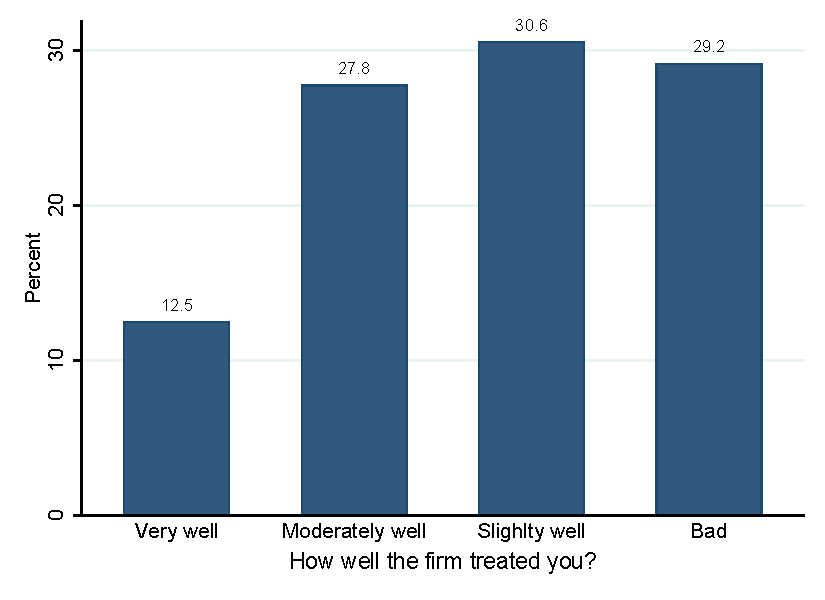
\includegraphics[width=\textwidth]{paper/Figuras/catplot_trato.pdf}
    \end{subfigure}
    \begin{subfigure}{0.475\textwidth}
        \caption{How common the firm treats bad their employees?}
        \centering
        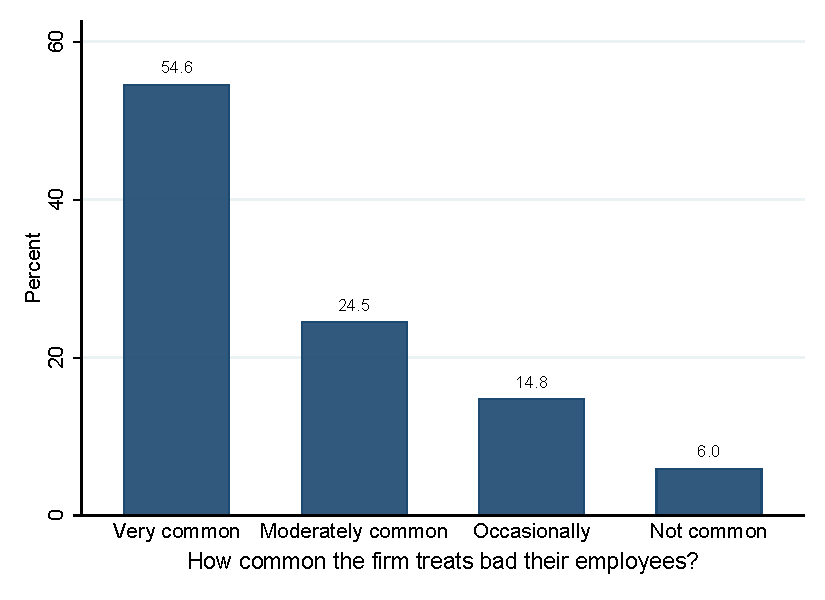
\includegraphics[width=\textwidth]{paper/Figuras/catplot_comun.pdf}
    \end{subfigure}
    \begin{subfigure}{0.475\textwidth}
        \caption{What's your level of anger towards the firm?}
        \centering
        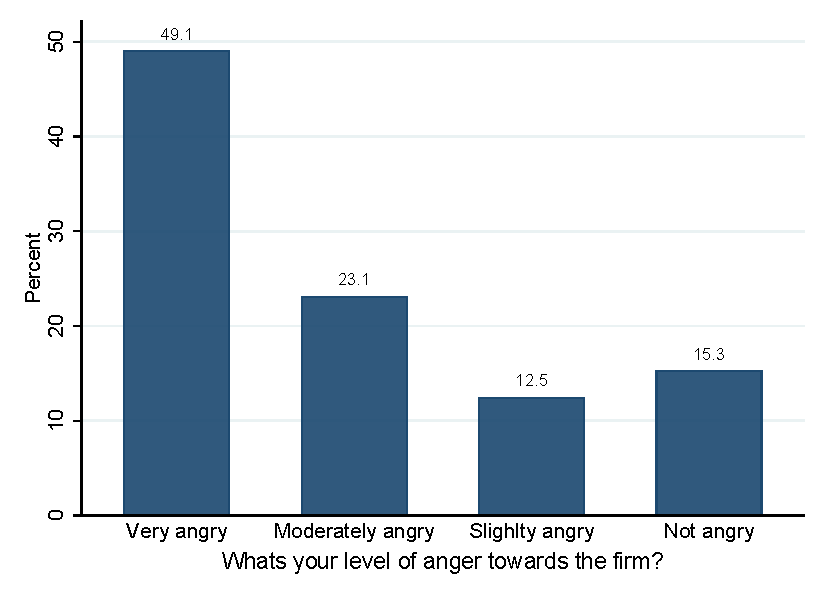
\includegraphics[width=\textwidth]{paper/Figuras/catplot_enojo.pdf}
    \end{subfigure}    
    \end{center}
    
    
\end{figure}

\begin{figure}[H]
    \caption{Interaction of emotions}
    \label{}
    \begin{center}

    \begin{subfigure}{0.475\textwidth}
        \caption{Commonly treated bad $\times$ Treated bad}
        \centering
        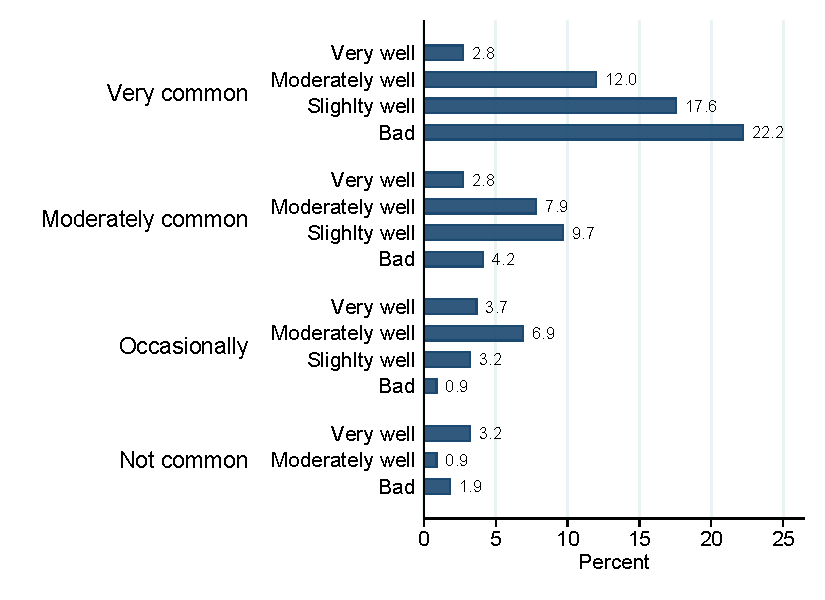
\includegraphics[width=\textwidth]{paper/Figuras/catplot_trato_comun.pdf}
    \end{subfigure}
    \begin{subfigure}{0.475\textwidth}
        \caption{Treated bad $\times$ Anger}
        \centering
        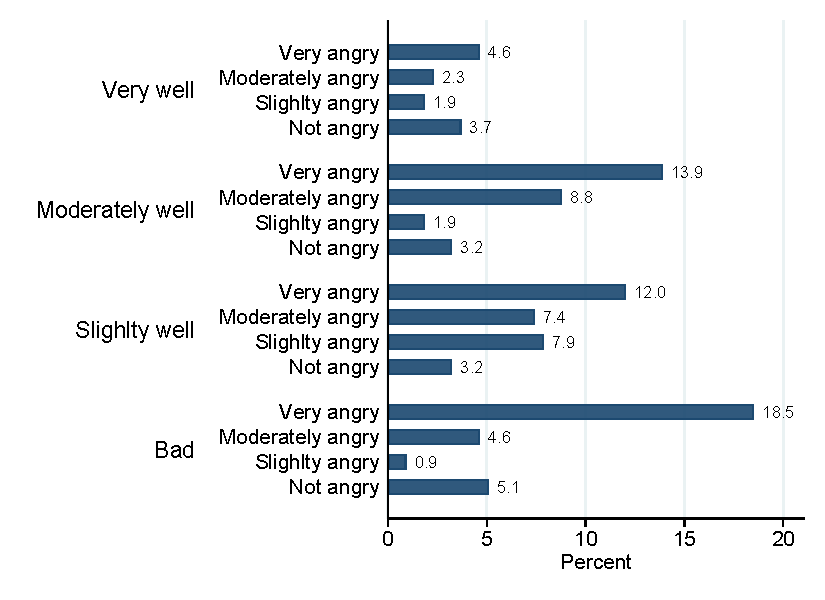
\includegraphics[width=\textwidth]{paper/Figuras/catplot_trato_enojo.pdf}
    \end{subfigure}
    \end{center}
    
    \scriptsize \textit{Notes:} Panel (a) interacts the two questions : How common the firm treats bad their employees? with How the firm treated the dismissed employee. Panel (b) interacts whether the employee was treated bad with her level of anger towards the firm.
    
\end{figure}

\newpage

\begin{landscape}
\section{Regressions}
%#include
\begin{table}[!ht]
    \caption{Correlation between emotions and bargaining}
    \label{tab:TreatmentArms}
    \begin{center}
     \scriptsize{% Table generated by Excel2LaTeX from sheet 'emotions_bargaining'
\begin{tabular}{lcccccccccccccccccccc}
\toprule
      & \multicolumn{6}{c}{Settlement}                &       & \multicolumn{6}{c}{Probability of winning}    &       & \multicolumn{6}{c}{Minimum amount to dismiss (IHS)} \\
\cmidrule{2-7}\cmidrule{9-14}\cmidrule{16-21}      & (1)   & (2)   & (3)   & (4)   & (5)   & (6)   &       & (7)   & (8)   & (9)   & (10)  & (11)  & (12)  &       & (13)  & (14)  & (15)  & (16)  & (17)  & (18) \\
\midrule
Treated bad & -0.11* & -0.17** &       &       & -0.083 & -0.076 &       & -5.12 & -8.76* &       &       & 10.6  & 10.3  &       & -0.40 & -0.78 &       &       & 1.24  & 2.53 \\
      & (0.064) & (0.065) &       &       & (0.15) & (0.17) &       & (4.04) & (4.43) &       &       & (9.33) & (10.3) &       & (0.77) & (0.87) &       &       & (2.61) & (2.98) \\
Angry &       &       & -0.082 & -0.11 & -0.072 & -0.077 &       &       &       & -6.75 & -6.88 & -0.53 & 0.96  &       &       &       & 0.43  & 1.10  & 1.08  & 2.45* \\
      &       &       & (0.080) & (0.085) & (0.092) & (0.097) &       &       &       & (5.09) & (5.53) & (7.03) & (8.10) &       &       &       & (1.17) & (1.20) & (1.34) & (1.47) \\
Treated bad $\times$ Angry &       &       &       &       & -0.034 & -0.11 &       &       &       &       &       & -20.0* & -24.1** &       &       &       &       &       & -2.06 & -4.18 \\
      &       &       &       &       & (0.17) & (0.19) &       &       &       &       &       & (11.3) & (11.9) &       &       &       &       &       & (2.88) & (3.19) \\
      &       &       &       &       &       &       &       &       &       &       &       &       &       &       &       &       &       &       &       &  \\
\midrule
Observations & 207   & 182   & 207   & 182   & 207   & 182   &       & 207   & 182   & 207   & 182   & 207   & 182   &       & 207   & 182   & 207   & 182   & 207   & 182 \\
R-sq  & 0.249 & 0.318 & 0.239 & 0.294 & 0.256 & 0.332 &       & 0.350 & 0.437 & 0.352 & 0.426 & 0.375 & 0.467 &       & 0.305 & 0.380 & 0.305 & 0.382 & 0.310 & 0.406 \\
DepVarMean & 0.11  & 0.12  & 0.11  & 0.12  & 0.11  & 0.12  &       & 79.3  & 78.1  & 79.3  & 78.1  & 79.3  & 78.1  &       & 9.48  & 9.68  & 9.48  & 9.68  & 9.48  & 9.68 \\
BVC + casefile controls &       & \checkmark &       & \checkmark &       & \checkmark &       &       & \checkmark &       & \checkmark &       & \checkmark &       &       & \checkmark &       & \checkmark &       & \checkmark \\
\midrule
\midrule
      &       &       &       &       &       &       &       &       &       &       &       &       &       &       &       &       &       &       &       &  \\
\midrule
      & \multicolumn{6}{c}{Minimum amount (IHS)}      &       & \multicolumn{6}{c}{Maximum amount (IHS)}      &       & \multicolumn{6}{c}{Most probable amount (IHS)} \\
\cmidrule{2-7}\cmidrule{9-14}\cmidrule{16-21}      & (19)  & (20)  & (21)  & (22)  & (23)  & (24)  &       & (25)  & (26)  & (27)  & (28)  & (29)  & (30)  &       & (31)  & (32)  & (33)  & (34)  & (35)  & (36) \\
\midrule
Treated bad & -1.36 & -1.90* &       &       & -4.42* & -3.04 &       & -1.43 & -1.98* &       &       & -4.39* & -2.90 &       & -1.39 & -1.93* &       &       & -4.40* & -2.95 \\
      & (0.87) & (0.99) &       &       & (2.35) & (2.71) &       & (0.90) & (1.03) &       &       & (2.47) & (2.86) &       & (0.88) & (1.00) &       &       & (2.41) & (2.77) \\
Angry &       &       & 0.95  & 1.84  & -0.29 & 1.39  &       &       &       & 1.07  & 2.02  & -0.13 & 1.66  &       &       &       & 0.94  & 1.86  & -0.28 & 1.46 \\
      &       &       & (1.19) & (1.20) & (1.41) & (1.48) &       &       &       & (1.24) & (1.25) & (1.44) & (1.53) &       &       &       & (1.21) & (1.22) & (1.42) & (1.49) \\
Treated bad $\times$ Angry &       &       &       &       & 3.88  & 1.42  &       &       &       &       &       & 3.75  & 1.16  &       &       &       &       &       & 3.80  & 1.27 \\
      &       &       &       &       & (2.79) & (3.08) &       &       &       &       &       & (2.93) & (3.25) &       &       &       &       &       & (2.86) & (3.16) \\
      &       &       &       &       &       &       &       &       &       &       &       &       &       &       &       &       &       &       &       &  \\
\midrule
Observations & 207   & 182   & 207   & 182   & 207   & 182   &       & 207   & 182   & 207   & 182   & 207   & 182   &       & 207   & 182   & 207   & 182   & 207   & 182 \\
R-sq  & 0.343 & 0.432 & 0.337 & 0.425 & 0.359 & 0.448 &       & 0.332 & 0.417 & 0.326 & 0.411 & 0.347 & 0.434 &       & 0.333 & 0.423 & 0.325 & 0.415 & 0.347 & 0.438 \\
DepVarMean & 8.32  & 8.53  & 8.32  & 8.53  & 8.32  & 8.53  &       & 8.73  & 8.93  & 8.73  & 8.93  & 8.73  & 8.93  &       & 8.50  & 8.68  & 8.50  & 8.68  & 8.50  & 8.68 \\
BVC + casefile controls &       & \checkmark &       & \checkmark &       & \checkmark &       &       & \checkmark &       & \checkmark &       & \checkmark &       &       & \checkmark &       & \checkmark &       & \checkmark \\
\bottomrule
\bottomrule
\end{tabular}%
}
     \end{center}
    
     \scriptsize
%\begin{figurenotes}
\textit{Notes:} This table shows correlation between outcomes (settlement) and the employee's expectation on outcomes with levels of emotions. The variable \textit{Treated bad} is coded as $1$ whenever respondent answers "Slightly well" or "Bad" to the question "How well the firm treated you?". The variable \textit{Angry} is defined to be $0$ only when respondent answer "Not angry" to the level of anger she experiences.  
%\end{figurenotes}    
\end{table}
\end{landscape} 



\end{document}


